\documentclass[oneside,spanish]{amsart}
\usepackage[T1]{fontenc} % Tipo de fuente
\usepackage[utf8]{inputenc} % Archivo UTF-8
\usepackage[a4paper]{geometry}
\geometry{verbose,tmargin=2cm,bmargin=2cm,lmargin=3cm,rmargin=2.5cm} % Tamaño
\usepackage{amsthm} 
%\usepackage{amsaddr} % Para modificar la posición de address
\usepackage[spanish]{babel} % Idioma español
\usepackage[backend=biber,style=alphabetic,natbib,maxalphanames=1]{biblatex} % Compilar bibliografía con BibLaTeX (no BibTeX)
\usepackage[shortlabels]{enumitem} % Mejora el entorno enumerate
\usepackage{graphicx} % Colocar imágenes
\usepackage[hidelinks]{hyperref} % Vínculos y referencias interactivas
\usepackage[skip=3pt]{caption} % Permite modificar el espacio entre el caption y la imagen
\usepackage{multicol} % Entornos de múltiples columnas

%-------------------------------------------------------------------------
% Configuraciones iniciales
\makeatletter
%Numeración
\numberwithin{equation}{section}
\numberwithin{figure}{section}
\newlength{\lyxlabelwidth}      % Longitud auxiliar
\makeatother
%-------------------------------------------------------------------------

%-------------------------------------------------------------------------
% Bibliografía
\defbibheading{bibliography}[\refname]{}
\addbibresource{refs-tall02.bib}

\renewcommand*{\labelalphaothers}{}

\DeclareLabelalphaTemplate{
	\labelelement{
		\field[final]{shorthand}
		\field{labelname}
		\field{label}
	}
	\labelelement{
		\literal{,\addhighpenspace}
	}
	\labelelement{
		\field{year}
	}
}
%-------------------------------------------------------------------------

%-------------------------------------------------------------------------
% Otras configuraciones
%\pagestyle{plain} % Para que el encabezado esté vacío
\addto\captionsspanish{\renewcommand{\tablename}{Tabla}}
\addto\captionsspanish{\renewcommand{\figurename}{Imagen}}
%-------------------------------------------------------------------------

\usepackage{fancyhdr}
\pagestyle{fancy}
\fancyhf{} % sets both header and footer to nothing
\renewcommand{\headrulewidth}{0pt}
\fancyhead[C]{\scriptsize\MakeUppercase\shorttitle}

%-------------------------------------------------------------------------

% Y acá comienza el documento

\begin{document}

%-------------------------------------------------------------------------
% Datos del artículo
\title[Visualización y uso de registros semióticos en trigonometría]{Comprensión de algunas nociones básicas de  trigonometría enfatizando la  visualización y uso de registros semióticos de representación\vspace{-2ex}}
\author[1]{Daniela Betsabé Alvarez\textsuperscript{1}}
\address[1]{Universidad Nacional de Salta. Sede Regional Orán}
\author[2]{Edith Marcela Chorolque}
\author[3]{Celia Elizabeth Villagra}
\author[4]{Isabel Hortensia Miguez}
\email[1]{danbet@hotmail.es}
%-------------------------------------------------------------------------

\begin{abstract}
	  La trigonometría es un tópico en el que la mayoría de los estudiantes del nivel medio tienen dificultades para la comprensión del mismo. Algunas investigaciones como la de \citet{torres-montiel-cuevas} y \citet{moore-k} consideran que es frecuente que los docentes tiendan a aritmetizar la trigonometría descuidando el contexto geométrico que proporciona el círculo trigonométrico. En este taller se revisarán los errores y dificultades más frecuentes de los estudiantes, analizando los obstáculos epistemológicos y didácticos que podrían provocarlos. Además, teniendo en cuenta que la trigonometría vincula diferentes tipos de pensamientos matemáticos: geométrico, métrico, algebraico y variacional, se propondrá hacer uso de los distintos registros semióticos definidos  por \citet{duval-r} para propiciar la significación de conceptos como circunferencia trigonométrica, funciones trigonométricas y ecuaciones trigonométricas. Se propondrán estrategias metodológicas que harán   hincapié en el proceso de visualización, como fuente de razonamiento deductivo, para favorecer la generalización, buscando que el estudiante sea capaz de realizar transformaciones y conversiones de registros de representación. Se utilizará el software dinámico Geogebra, ya que es  una herramienta fundamental que permitirá que el estudiante articule múltiples representaciones, explorando, relacionando y conjeturando y así favorecer el aprendizaje activo de la trigonometría.
\end{abstract}

\maketitle
\thispagestyle{empty}

\section{Contenidos}

Errores y dificultades en la enseñanza y aprendizaje de la trigonometría. Pensamiento matemático: geométrico, métrico, algebraico y variacional. La visualización en matemática. Teoría de las representaciones semióticas de Duval. Circunferencia trigonométrica y goniométrica. Funciones trigonométricas de un número real. Ecuaciones trigonométricas. Uso de Tic´s: Geogebra.

\section{Requisitos Previos}

Uso de herramientas de geometría y de funciones de Geogebra. Conocimiento de razones trigonométricas y circunferencia trigonométrica.

\section{Objetivos}

Reconocer y analizar errores y dificultades más frecuentes de los estudiantes cuando resuelven  situaciones vinculadas a la trigonometría.

Valorar el uso de los diferentes registros semióticos de representación para promover la significación de algunos conceptos en trigonometría.

Incorporar el Geogebra como herramienta que potencia la coordinación de múltiples registros de representación posibilitando la comprensión de conceptos en trigonometría.

\section{Actividades}

\subsection{Actividades Previas}

Se proponen dos actividades consistentes en cuestionarios. Se indicará que si aún no ha enseñado trigonometría o no tiene experiencia como docente, que se apoye en su trayectoria como estudiante del nivel medio o como practicante en una escuela asociada, para responder el mismo.

A continuación se muestran las actividades previas propuestas:

\paragraph{Actividad 1:}

Teniendo en cuenta que \citet{godino-batanero-font} destacan la diferenciación existente entre los términos \textit{error} y \textit{dificultad}. Mientras el error se refiere a si “una práctica es válida o no desde el punto de vista de la institución escolar”, la dificultad se refiere al “mayor o menor grado de éxito de los alumnos ante una tarea o tema de estudio”. Por ejemplo, un error frecuente  cuando resuelven ecuaciones es que transponen como un término positivo a un factor negativo. Una dificultad en la resolución de ecuaciones es que los estudiantes no tienen dominio de las operaciones con números enteros o racionales. Responda:

\begin{enumerate}[a.]
	\item ¿Cuáles son algunos errores frecuentes que cometen los estudiantes cuando resuelven actividades vinculadas a la trigonometría?
	
	\item ¿Qué dificultades puede identificar en el aprendizaje de la trigonometría?
	
	\item Observe el siguiente gráfico de la función seno realizado por una estudiante, identifique errores en el mismo. $f(x)= \sen x$
\end{enumerate}

\bigskip

\paragraph{Actividad 2:}

Responda:

\begin{enumerate}[2.1.]
	\item ¿Considera que la trigonometría es de difícil comprensión para los estudiantes? ¿por qué?
	
	Teniendo en cuenta los diseños curriculares de Matemática de su provincia, para ciclo básico y superior del nivel medio y escuelas técnicas (se anexa una tabla para la provincia de Salta).
	\begin{enumerate}[a.]
		\item ¿Cuáles contenidos se desarrollan en su escuela?
		\item Si no se desarrollan todos los contenidos. ¿Cuál será el motivo?
	\end{enumerate}
	
	\item ¿Utiliza algún software para la enseñanza de temas de trigonometría?, ¿cuál? ¿Y para qué temas de trigonometría  lo utiliza?
\end{enumerate}

\subsection{Primeras dos horas sincrónicas}\label{subsec:primeras-dos}

\paragraph{Contenidos:}

Errores y dificultades en la enseñanza de la trigonometría. Pensamiento matemático. La visualización en matemática. Circunferencia trigonométrica.

\begin{enumerate}
	\item Se recuperarán las respuestas de la actividad previa para sistematizar errores y dificultades identificados.
	\item Se presentará a través de una presentación en Power Point los errores y dificultades aportados por las investigaciones en la temática. Se diferenciará el origen epistemológico o didáctico de los mismos.
	\item Se presentará una actividad en el círculo trigonométrico propuesta por \citet{salazar-mendez}, que los docentes deberán resolver en grupos. Para la misma se utilizarán grupos en la plataforma Zoom, los talleristas recorrerán los mismos para orientar y recabar información sobre la solución que proponen. Posteriormente se realiza una puesta en común con al menos dos resoluciones diferentes. 
	\item Un tallerista realizará el cierre de la actividad haciendo hincapié en la visualización y presentando  a través de Power Point el marco teórico de pensamiento matemático y proceso de visualización.
\end{enumerate}

\subsection{Primeras dos horas entre clases}\label{subsec:primeras-dos-EC}

\paragraph{Contenidos:} visualización. Registros semióticos de representación de Duval. Circunferencia trigonométrica y goniométrica.

\begin{enumerate}[1.]
	\item Se proporcionará un texto resumido sobre los registros semióticos de representación semiótica de Duval que los cursantes deben leer.
	\item Se mostrará la actividad completa propuesta por \citet[pág. 73]{salazar-mendez} . Deberán resolverla usando Geogebra e identificar registros, transformaciones y conversiones. (se transcribe parte de la actividad).
	
	\hspace{1mm}
	
	\begin{enumerate}[1.]
	\item Abra el archivo “\textit{Tarea 1}”. Arrastre el punto B y observe lo que sucede. A continuación (Tabla \ref{tab:imagen1}).
		
	\begin{table}[h]
		\centering
		\caption{}
		\label{tab:imagen1}
		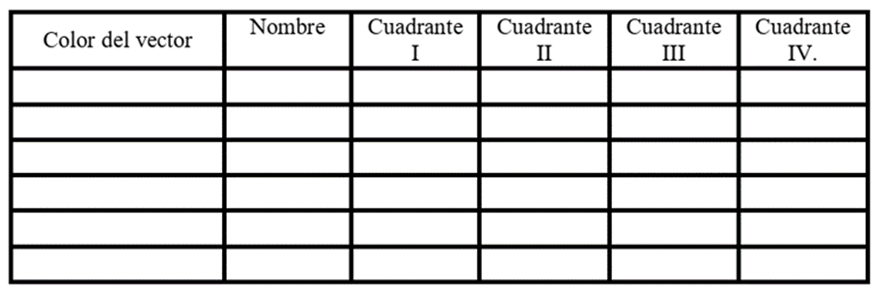
\includegraphics[width=0.8\linewidth]{Anexos-02/Imagen1.png}
	\end{table}
		
	\begin{enumerate}[a.]
		\item Determine el signo de cada vector (diferenciándolos por color y nombre) en cada cuadrante del plano cartesiano:
			
		Puedes observar cómo cambia el ángulo central y la medida de cada vector. Explica:
			
		\item Cuando arrastras el punto $B$, ¿Qué cambios se presentan en el vector $CD$ cada vez que cambia la medida del ángulo central?
			
		\item ¿Qué sucede con este vector cuando se sobrepone el punto $B$ sobre el punto $E$ y sobre $E'$? Explica. ¿Cuántos grados mide el ángulo central en cada una de estas posiciones?
		\end{enumerate}
		
	\item Encuentra la longitud de cada vector y registra los datos en la siguiente tabla, asociando los colores similares. Arrastrando el punto B, regístralos 3 veces, (Tabla \ref{tab:imagen2}).
	
	\begin{table}[h]
		\centering
		\caption{}
		\label{tab:imagen2}
		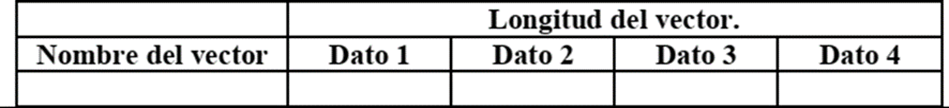
\includegraphics[width=0.8\linewidth]{Anexos-02/Imagen2.png}
	\end{table}
	\end{enumerate}
\end{enumerate}	

\break

\subsection{Segundas dos horas sincrónicas}\label{subsec:segundas-dos}

\paragraph{Contenidos:}

Teoría de las representaciones semióticas de Duval. Circunferencia trigonométrica. Funciones trigonométricas de un número real. Uso de Geogebra.

\begin{enumerate}[1.]
	\item Se realizarán preguntas para indagar sobre la comprensión de registros semióticos y acerca de las operaciones de transformación y conversión. Se aclararán dudas si fuera necesario.
	\item Se recordarán algunas herramientas básicas para funciones en Geogebra.
	\item Se resolverán una actividad  grupal  en Geogebra que permitirá caracterizar las funciones seno y coseno, período y amplitud. Para ello se utilizará una actividad publicada en el sitio web de Geogebra\footnote{\url{https://www.geogebra.org/m/HdnfNmwA}} y a un grupo se le solicitará estudiar la función seno, a otro la función coseno y a un tercer grupo la función tangente. Esta actividad contará con una serie de preguntas que posibilitarán la exploración e investigación.
	\item Se realizará una puesta en común haciendo hincapié en los registros y la necesidad de cambio de registro para responder las preguntas.
\end{enumerate}

\subsection{Segundas dos horas Entre Clases}\label{subsec:segundas-dos-EC}

\paragraph{Contenidos:}

Funciones trigonométricas. Ecuaciones trigonométricas. Uso de Geogebra.

\begin{enumerate}[1.]
	\item Resolución de una actividad sobre funciones trigonométricas usando Geogebra. (para ello se acompaña un pequeño tutorial recordando herramientas básicas para uso de Geogebra con funciones).
	\item Se les mostrará cómo se puede resolver una ecuación trigonométrica utilizando el registro gráfico (circunferencia trigonométrica) y cómo luego verifican usando registro numérico. Se les pedirá que resuelvan cuatro ecuaciones trigonométricas utilizando la circunferencia trigonométrica.
\end{enumerate}

\subsection{Terceras dos horas sincrónicas}\label{terceras-dos}

\paragraph{Contenidos:}

Funciones trigonométricas. Ecuaciones trigonométricas. Uso de Geogebra.

\begin{enumerate}[1.]
	\item Se recupera la resolución de ecuaciones presentadas en la clase asincrónica.
	\item Se resuelve en grupo una actividad donde se vincula función trigonométrica con ecuaciones trigonométricas. 
	\item Se realiza la puesta en común.
	\item Un tallerista muestra cómo  se puede vincular registro gráfico en sistemas cartesianos con el registro algebraico y numérico al resolver ecuaciones. 
\end{enumerate} 

\subsection{Evaluación final}

Puede realizarse en grupos de hasta dos integrantes.

\paragraph{Actividad 1:}

Se les proporcionará una actividad de trigonometría donde deberán analizar contenidos vinculados, reconocer los registros semióticos que pueden utilizar los estudiantes , proponer la resolución de la actividad identificando transformaciones y conversiones. En la resolución debe hacer uso de Geogebra y presentar las capturas de pantallas.

\bigskip

\paragraph{Actividad 2:}

El docente deberá proponer una actividad de funciones trigonométricas o ecuaciones trigonométricas, donde sea necesario el uso de diferentes registros de representación semiótica.

\section{Bibliografía}

\printbibliography

\end{document}